\documentclass[11pt,a4paper]{article}
\usepackage[top=3cm, bottom=2cm, left=2cm, right=2cm]{geometry}
\usepackage[utf8]{inputenc}
\usepackage{amsmath, amsfonts, amssymb}
\usepackage{siunitx}
\usepackage[brazil]{babel}
\usepackage{graphicx}
\usepackage[margin=10pt,font={small, it},labelfont=bf, textfont=it]{caption}
\usepackage[dvipsnames, svgnames]{xcolor}
\DeclareCaptionFont{MediumOrchid}{\color[svgnames]{MediumOrchid}}
\usepackage[pdftex]{hyperref}
\usepackage{natbib}
\bibliographystyle{plainnat}
\bibpunct{[}{]}{,}{s}{}{}
\usepackage{color}
\usepackage{footnote}
\usepackage{setspace}
\usepackage{booktabs}
\usepackage{multirow}
\usepackage{subfigure}
\usepackage{fancyhdr}
\usepackage{leading}
\usepackage{indentfirst}
\usepackage{wrapfig}
\usepackage{mdframed}
\usepackage{etoolbox}
\usepackage[version=4]{mhchem}
\usepackage{enumitem}
\usepackage{caption}
\usepackage{titlesec}
\usepackage{tcolorbox}
\usepackage{tikz}
\usepackage{LobsterTwo}
\usepackage[T1]{fontenc}
\usepackage{fontspec}
\usepackage{txfonts}
\AtBeginEnvironment{equation}{\fontsize{13}{16}\selectfont}


\titleformat{\section}{\LobsterTwo\LARGE\color{CarnationPink}}{\thesection.}{1em}{}
\titleformat{\subsection}{\LobsterTwo\LARGE\color{CarnationPink}}{\thesubsection}{1em}{}


\DeclareCaptionLabelFormat{figuras}{\textcolor{DarkTurquoise}{Figura \arabic{figure}}}
\captionsetup[figure]{labelformat=figuras}

\makeatletter
\renewcommand\tagform@[1]{\maketag@@@{\color{CarnationPink}(#1)}}
\makeatother

\renewcommand{\theequation}{Eq. \arabic{equation}}
\renewcommand{\thefigure}{Fig. \arabic{figure}}
\renewcommand{\thesection}{\textcolor{CarnationPink}{\arabic{section}}}

\setlist[itemize]{label=\textcolor{CarnationPink}{$\mathbf{\square}$}}

\setlist[enumerate]{label=\textcolor{CarnationPink}{\arabic*.}, align=left, leftmargin=1.5cm}


\newcounter{exemplo}

\NewDocumentEnvironment{exemplo}{ O{} }{%
\allowbreak
\setlength{\parindent}{0pt}
  \begin{mdframed}[
  leftline=true,
  topline=false,
  rightline=false,
  bottomline=false,
  linewidth=2pt,
  linecolor=CarnationPink,
  frametitlerule=false,
  frametitlefont=\LobsterTwo\large\color{CarnationPink},
  frametitle={\color{CarnationPink}\LobsterTwo\large #1},
  ]
}{%
  \end{mdframed}
}

\setlength{\fboxsep}{5pt}
\setlength{\fboxrule}{1.5pt}
\usepackage{float}
\renewcommand{\thefootnote}{\alph{footnote}}
\usepackage{url}
\hypersetup{
	colorlinks=true,
	linkcolor=DarkTurquoise,
	filecolor=DarkTurquoise,      
	urlcolor=DarkTurquoise,
	citecolor=DarkTurquoise,
	pdftitle={Especialista em Física da Radioterapia}
}
\pagestyle{fancy}
\fancyhf{}
\renewcommand{\headrulewidth}{0pt}
\rfoot{Página \thepage}

\title{\LobsterTwo\Huge{Radioterapia}}
\author{\LobsterTwo\Large{Teleterapia com Feixes de Elétrons}\nocite{*}}
\date{\LobsterTwo\textit{Dalila Mendonça}}
\begin{document}
	\maketitle

\section{Introdução}

	Feixes de elétrons têm sido usados em radioterapia desde a década de 1940, mas não ganharam uso generalizado até a década de 1970 com o desenvolvimento comercial dos aceleradores lineares (linacs). Os elétrons perdem energia à medida que atravessam um meio através de várias colisões elásticas e inelásticas com elétrons atômicos e o núcleo. Colisões inelásticas com o núcleo resultam na perda radiativa de um fóton, chamada produção de bremsstrahlung.
	
	A radiação bremsstrahlung criada pelas interações do feixe de elétrons com folhas de espalhamento de alto número atômico e outros materiais no caminho do feixe é chamada de contaminação de fótons. Os elétrons são uma partícula carregada com um alcance finito e, portanto, são adequados para o tratamento de alvos mais superficiais.

	Como se tratam de partículas carregadas, os elétrons de megavoltagem sofrem mais espalhamento do que os fótons de megavoltagem, particularmente no ar. É por isso que os feixes de elétrons usam cones com trimmers de feixe bem próximos à superfície do paciente para minimizar o espalhamento dos elétrons para fora do campo de tratamento. Para personalizar ainda mais a forma do feixe, os recortes cerrobend são colocados no topo dos trimmers (cutouts).

	O forma como ocorre o espalhamento dos elétrons muda com a energia inicial do elétron e com a profundidade no meio. Isso dificulta o matching de campos adjacentes de elétrons com outros campos de elétrons ou com campos de fótons. As muitas fontes de espalhamento no caminho do feixe de elétrons (folhas de espalhamento, câmaras monitoras, cone de elétrons) também afetam a dependência da distância da saída do feixe. O conceito de uma posição de fonte efetiva é usado para descrever isso.

	Três fatores que afetam grandemente a distribuição da dose dos feixes de elétrons são:
	
	\begin{enumerate}
		\item a obliquidade do feixe;
		\item a irregularidade da superfície; e
		\item a falta de homogeneidade do tecido.
	\end{enumerate}
	
	Os algoritmos pencil beam tradicionais não calculam com precisão a dose nessas condições. Os cálculos de Monte Carlo para elétrons estão se tornando cada vez mais comuns e funcionam muito melhor nessas condições.

	O AAPM TG-70, \textit{\textbf{``Recommendations for Clinical Electron Beam Dosimetry''}}, produziu um suplemento para o AAPM TG-25, \textit{\textbf{``Clinical Electron Beam Dosimetry''}}, que atualizou as seções de dosimetria absoluta para refletir a mudança na dose absorvida nos padrões de água. As discussões no AAPM TG-25 sobre obliquidade, dose de superfície, posição efetiva da fonte, correções de gap de ar e uso de diodos permanecem válidas. O relatório AAPM TG-70 apresenta uma discussão detalhada sobre o uso de elétrons em muitas situações clínicas.

\section{Características dos Feixes de Elétrons}

\subsection*{Porcentagem de Dose Na Profundidade}

	As curvas típicas de dose na profundidade para os feixe de elétrons são mostradas na \ref{fig:pdpeletrons}. Eles mostram uma dose de superfície relativamente alta em comparação com feixes de fótons com a mesma energia nominal, um acúmulo até a dose máxima, uma rápida queda na dose e, em seguida, um pequeno componente de baixa dose chamado cauda de bremsstrahlung ou contaminação de fótons. A contaminação de fótons aumenta com o aumento da energia, conforme mostrado na \ref{fig:pdpeletrons}.

	\begin{figure}[h]
		\centering
		\fcolorbox{DarkTurquoise}{white}{%
			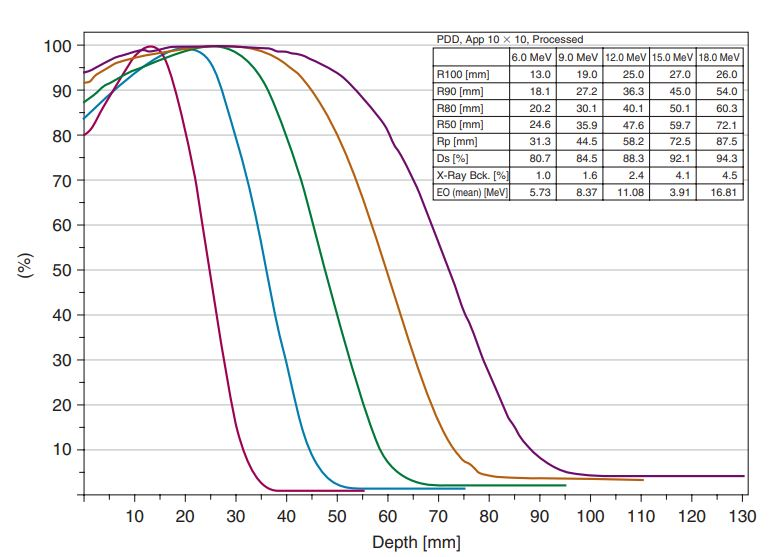
\includegraphics[width=0.8\textwidth]{Imagens/pdpeletrons.JPG}
		}%
		\caption{Exemplo de Curvas de PDP para feixes de Elétrons.}
		\label{fig:pdpeletrons}
	\end{figure}

	Existem vários parâmetros de dose na profundidade que são usados para descrever uma curva de dose de profundidade de elétrons: dose de superfície, profundidade de dose máxima (R100 ou $\mathrm{D_{max}}$), profundidade da isodose de 90\% (R90), profundidade da isodose de 80\% (R80), profundidade da isodose de 50\% (R50), alcance prático (Rp) e a contaminação por fótons.

	Os parâmetros de alcance das isodoses na profundidade mudam com o tamanho do campo, mas a mudança é pequena para tamanhos de campo maiores do que o alcance prático. De fato, os dados na literatura demonstram que para energias menores ou iguais a 16 MeV, as mudanças em qualquer um dos parâmetros de alcance são menores que 1 mm para os cones de 10 cm x 10 cm até os cones de 25 cm x 25 cm. Para energias menores ou iguais a 12 MeV, isso se estende até o cone de 6 cm x 6 cm. Um exemplo da alteração do R90 em função do tamanho de campo é apresentado na \ref{fig:r90}.
	
	\begin{figure}[h]
		\centering
		\fcolorbox{DarkTurquoise}{white}{%
			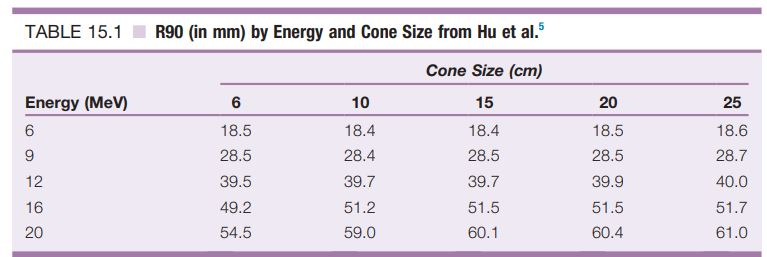
\includegraphics[width=0.7\textwidth]{Imagens/r90.JPG}
		}%
		\caption{R90 (em mm) em função da energia e do tamanho do cone.}
		\label{fig:r90}
	\end{figure}
	
	Para energias mais altas pode haver diferenças significativas, como mostra a \ref{fig:pdpeletronsECampo}. Para elétrons, a dose de superfície aumenta com a energia, o que é o oposto de fótons, e também pode ser observado na \ref{fig:pdpeletrons}.

	\begin{figure}[h]
		\centering
		\fcolorbox{DarkTurquoise}{white}{%
			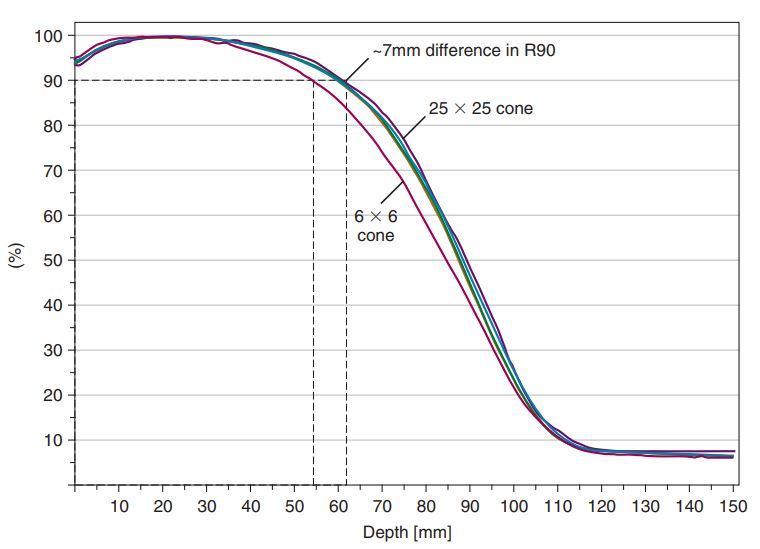
\includegraphics[width=0.8\textwidth]{Imagens/pdpeletronsECampo.JPG}
		}%
		\caption{Exemplo de mudança da PDP com diminuição do tamanho do cone para um elétron de maior energia (22 MeV).}
		\label{fig:pdpeletronsECampo}
	\end{figure}

	A \ref{fig:estimarOsRs} apresenta regras gerais que podem ser usadas para estimar os parâmetros de alcance. Estas regras destinam-se a ser estimativas rápidas e não podem substituir os dados medidos. Os valores podem diferir ligeiramente entre os linacs de diferentes modelos. Na prática clínica, esses valores devem ser tabelados em um formato conveniente semelhante à tabela da \ref{fig:pdpeletrons} e disponibilizados prontamente aos médicos como um auxílio na escolha da energia do feixe. Na prática clínica, a energia é frequentemente selecionada de modo que a profundidade R90 seja no mínimo tão profunda quanto o a região mais distal do volume alvo (PTV). A energia também deve ser limitada para reduzir a dose em quaisquer tecidos ou órgãos de risco (OARs) distais ao alvo.

	\begin{figure}[h]
		\centering
		\fcolorbox{DarkTurquoise}{white}{%
			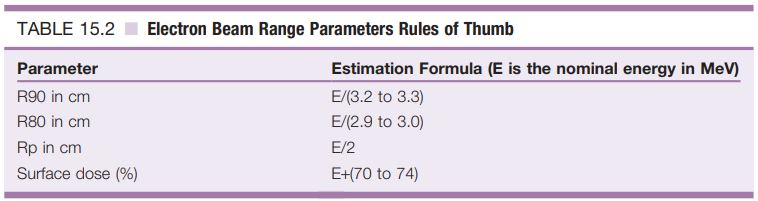
\includegraphics[width=0.8\textwidth]{Imagens/estimarOsRs.JPG}
		}%
		\caption{Regras práticas para estimar os parâmetros de alcance do feixe de elétrons.}
		\label{fig:estimarOsRs}
	\end{figure}

\subsection*{Output e Cutouts}

	A tendência de output dos cones de elétrons varia de acordo com a energia. O Centro de Física Radiológica (RPC), agora IROC Houston, publicou dados de referência para muitos modelos de linacs. Um exemplo do conjunto de dados é mostrado na Figura 15.3. Como mencionado acima, a dose de profundidade permanece inalterada para tamanhos de campo maiores do que a faixa prática. Da mesma forma, há pouca mudança na saída de um feixe de elétrons até tamanhos de corte iguais ao alcance prático. Dado que Rp pode ser estimado por E/2, isso implica que apenas campos menores que 3 cm para um feixe de 6 MeV terão mudanças significativas. Esta é apenas uma estimativa, e a validade de um determinado linac deve ser estabelecida no momento do comissionamento.

	\begin{figure}[h]
		\centering
		\fcolorbox{DarkTurquoise}{white}{%
			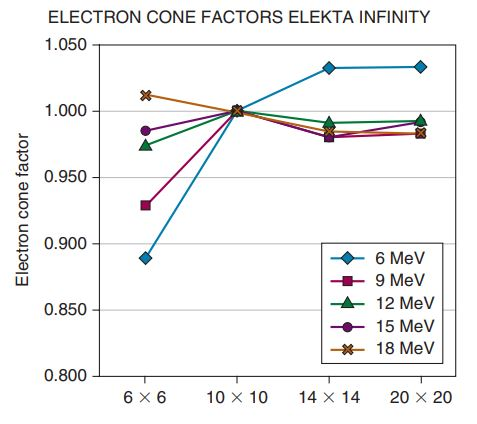
\includegraphics[width=0.8\textwidth]{Imagens/fatorcone.JPG}
		}%
		\caption{Exemplo de fatores de output do cone de elétrons em função do tamanho do cone e da energia do feixe.}
		\label{fig:fatorcone}
	\end{figure}

\bibliography{ref.bib}
\end{document}